\documentclass[border=1cm]{standalone}
\usepackage{tikz}

\begin{document}
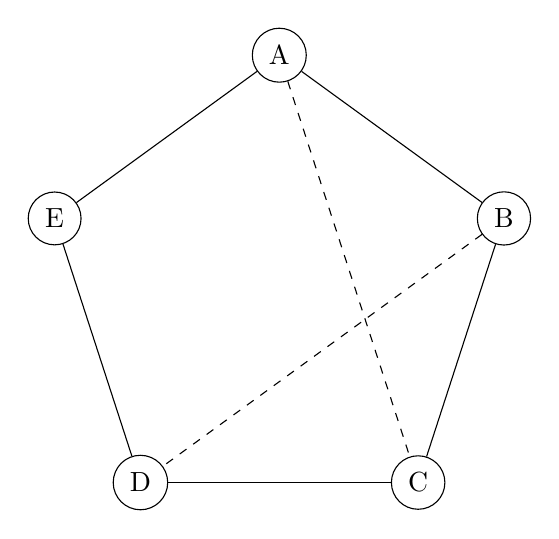
\begin{tikzpicture}[scale=2]

\def\r{1.5}% радиус окружности

\node[circle,draw] (A) at (90:\r) {A};
\node[circle,draw] (B) at (18:\r) {B};
\node[circle,draw] (C) at (-54:\r) {C};% узлы по окружности
\node[circle,draw] (D) at (-126:\r) {D};
\node[circle,draw] (E) at (162:\r) {E};

\draw (A) -- (B);
\draw (B) -- (C);
\draw (C) -- (D);% рёбра
\draw (D) -- (E);
\draw (E) -- (A);

\draw[dashed] (A) -- (C);% диагонали
\draw[dashed] (B) -- (D);

\end{tikzpicture}
\end{document}